\chapter{给生物分类}\label{ch:g3:sorting-living-things}

把一盒混在一起的纽扣倒在桌上，你的双手便会自动开始\omterm{def:g3:sorting-living-things:criterion}{分类}：大的和大的放在一起，
红的和红的放在一起，四个孔的和四个孔的
放在一起。博物学家面对\omterm{def:g1:living-or-not:living}{生物}世界中
甲虫、\omterm{prop:g3:sorting-living-things:groups}{鸟类}、蕨类和\omterm{prop:g3:sorting-living-things:groups}{鱼类}的纷繁杂陈，也有同样的冲动——
而仔细地给\omterm{def:g1:living-or-not:living}{生物}\omterm{def:g3:sorting-living-things:criterion}{分类}，
竟成为生物学最有力的思想之一。

\section{分类需要一个标准}

\begin{definition}[分类与标准]\label{def:g3:sorting-living-things:criterion}
把一组东西\emph{分类}\index{分类}，就是把
相互归属的东西放在一起。\emph{标准}\index{标准}是
分类所依据的规则——“有六条腿”“有\omterm{def:g1:animals-around-us:covering}{羽毛}”。对\omterm{def:g1:living-or-not:living}{生物}来说，好的标准是
身体的一种特征，它可以被\emph{观察}到：
即\omterm{def:g1:animals-around-us:animal}{动物}或\omterm{def:g1:plants-around-us:plant}{植物}自身
\emph{具有}的东西，而不是它住在哪里，或它恰好在做什么。
\end{definition}

\begin{example}[同一批动物的两种分类]\label{ex:g3:sorting-living-things:two}
取猫、鸭、鳟鱼和瓢虫。按
“生活在水边”来分：鸭和鳟鱼归为一组。按“有\omterm{def:g1:animals-around-us:covering}{羽毛}”来分：
只有鸭单独一类。两种都是\omterm{def:g3:sorting-living-things:criterion}{分类}，但只有
第二种利用了\omterm{def:g1:animals-around-us:animal}{动物}自身的身体特征，而这正是
生物学家所信赖的\omterm{def:g3:sorting-living-things:criterion}{分类}方式：\omterm{def:g1:animals-around-us:animal}{动物}可以搬家，却不能把
\omterm{def:g1:animals-around-us:covering}{羽毛}换成鳞片。
\end{example}

\begin{remark}[为什么不按住处或食物分类？]\label{rem:g3:sorting-living-things:why}
\omterm{def:g2:where-animals-live:habitat}{栖息地}和食物会随季节和运气而变化——
在\cref{ch:g2:what-animals-eat}中出现的乌鸫，会从吃蠕虫转为吃浆果，
而它并不会因此变成另一种\omterm{def:g1:animals-around-us:animal}{动物}。身体特征则保持不变。
因此，“它有什么”比“它做什么”更适合作为
\omterm{def:g3:sorting-living-things:criterion}{分类}的\omterm{def:g3:sorting-living-things:criterion}{标准}。
\end{remark}

\section{动物的几大类群}

\begin{proposition}[几个大类群]\label{prop:g3:sorting-living-things:groups}
按身体特征\omterm{def:g3:sorting-living-things:criterion}{分类}，可以把\omterm{def:g1:animals-around-us:animal}{动物}归入几个大类群，
包括：
\begin{itemize}
  \item \emph{昆虫}\index{昆虫}：六条腿，身体分为三
        部分——蚂蚁、瓢虫、蜜蜂、蝴蝶；
  \item \emph{鱼类}\index{鱼类}：有鳍和鳞片，一生生活在
        水中——鳟鱼、金鱼；
  \item \emph{鸟类}\index{鸟类}：有\omterm{def:g1:animals-around-us:covering}{羽毛}、翅膀和喙——
        鸭、乌鸫、鸵鸟；
  \item \emph{哺乳动物}\index{哺乳动物}：有\omterm{def:g1:animals-around-us:covering}{皮毛}或毛发，母体
        用\omterm{def:g2:animals-grow-up:born}{乳汁}喂养幼体——猫、牛、蝙蝠、
        鲸，以及人；
  \item \emph{两栖动物}\index{两栖动物}：\omterm{def:g1:the-five-senses:sense}{皮肤}湿润，卵产在
        水中，幼体为\omterm{ex:g2:animals-grow-up:frog}{蝌蚪}期——青蛙、蝾螈。
\end{itemize}
\end{proposition}
\admitted

\begin{omfigure}
\begin{tikzpicture}
  \foreach \x/\name/\feat in {
      0/昆虫/{6 条腿},
      2.95/鱼类/{鳍、鳞片},
      5.9/鸟类/{羽毛、喙},
      8.85/哺乳动物/{毛皮、乳汁},
      11.8/两栖动物/{湿润的皮肤}} {
    \draw[thick, omDef, fill=omDef!6, rounded corners=5pt]
      (\x,0) rectangle ({\x+2.8},1.7);
    \node[font=\small\bfseries, text height=1.6ex, text depth=0.4ex]
      at ({\x+1.4},1.3) {\name};
    \node[font=\small, text height=1.6ex, text depth=0.4ex]
      at ({\x+1.4},0.6) {\feat};
  }
\end{tikzpicture}

{\small 五个大类群，各以其成员所
\emph{具有}的特征命名。}
\end{omfigure}

\begin{example}[意外情形的正确判断]\label{ex:g3:sorting-living-things:surprises}
\omterm{def:g3:sorting-living-things:criterion}{标准}能让我们免于草率的猜测。蝙蝠飞起来像鸟——
但它有\omterm{def:g1:animals-around-us:covering}{皮毛}、没有\omterm{def:g1:animals-around-us:covering}{羽毛}，并用\omterm{def:g2:animals-grow-up:born}{乳汁}喂养幼体：是\omterm{prop:g3:sorting-living-things:groups}{哺乳动物}。
鲸游起来像鱼——\omterm{def:g1:animals-around-us:covering}{皮毛}几乎退化殆尽，但
用\omterm{def:g2:animals-grow-up:born}{乳汁}哺育幼崽，且没有鳞片：同样是\omterm{prop:g3:sorting-living-things:groups}{哺乳动物}。鸵鸟根本
不能飞，但\omterm{def:g1:animals-around-us:covering}{羽毛}和喙表明它是鸟。决定结论的是\omterm{def:g3:sorting-living-things:criterion}{标准}，
而不是第一印象。
\end{example}

\begin{omfigure}
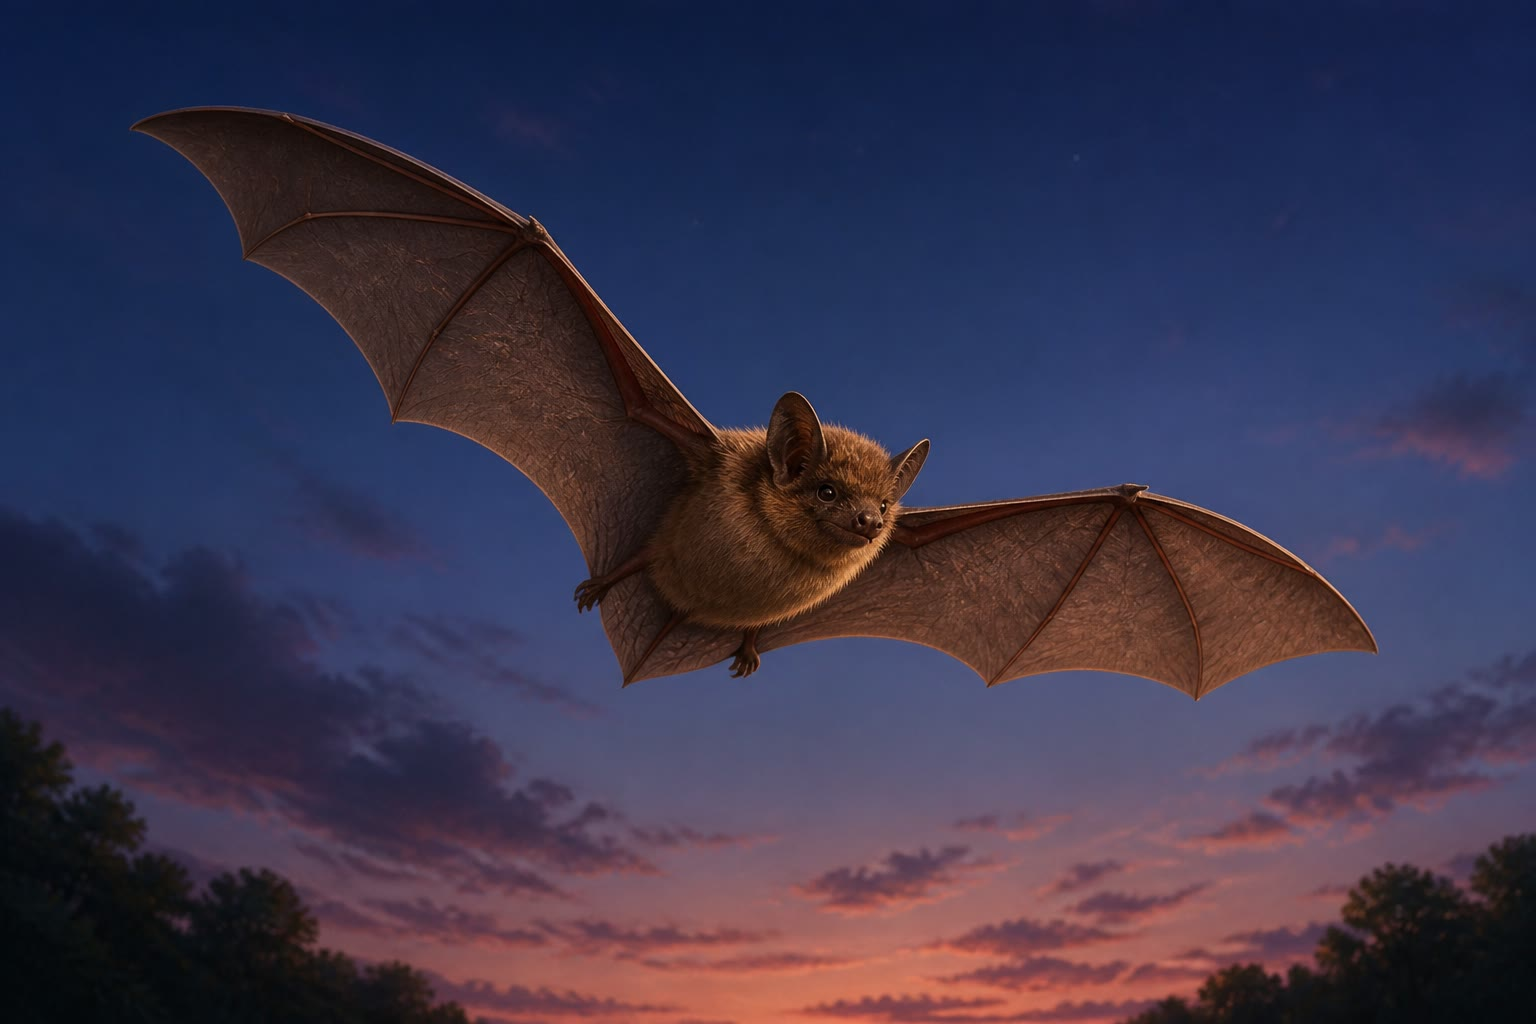
\includegraphics[width=0.6\linewidth]{images/book1/ai/g3-sort-bat.jpg}

{\small 它飞起来像鸟，裸露的翅膀上却长着\omterm{def:g1:animals-around-us:covering}{皮毛}：
蝙蝠，是按特征而非印象\omterm{def:g3:sorting-living-things:criterion}{分类}的
经典例子。}
\end{omfigure}

\begin{method}[给一种陌生动物分类]\label{met:g3:sorting-living-things:sort}
\begin{enumerate}
  \item 观察身体：是\omterm{def:g1:the-five-senses:sense}{皮肤}、\omterm{def:g1:animals-around-us:covering}{皮毛}、\omterm{def:g1:animals-around-us:covering}{羽毛}还是鳞片？有几条
        腿？有翅膀吗？有喙吗？
  \item 如果可以，问问幼体的情况：是否哺乳？是否产卵？
        是否经历\omterm{ex:g2:animals-grow-up:frog}{蝌蚪}期？
  \item 对照
        \cref{prop:g3:sorting-living-things:groups}中的各类群，
        把\omterm{def:g1:animals-around-us:animal}{动物}放入与其\emph{特征}相符的那一类；
  \item 若印象（“它会飞！”）与某一特征（
        “它有\omterm{def:g1:animals-around-us:covering}{皮毛}”）相矛盾，则以特征为准。
\end{enumerate}
\end{method}

\section{植物也要分类}

\begin{proposition}[植物的分类]\label{prop:g3:sorting-living-things:plants}
\omterm{def:g1:plants-around-us:plant}{植物}和\omterm{def:g1:animals-around-us:animal}{动物}一样，也依据其特征\omterm{def:g3:sorting-living-things:criterion}{分类}。有用的
\omterm{def:g3:sorting-living-things:criterion}{标准}有：它是否开\emph{花}、结\omterm{def:g2:from-seed-to-plant:seed}{种子}（如雏菊、
栗树），还是从不开花结籽（如蕨类、苔藓）？茎是否柔软、
呈绿色，还是像\emph{树}的树干一样木质化？\omterm{def:g1:plants-around-us:parts}{叶子}是宽阔的，
还是像松树那样的针形叶？
\end{proposition}
\admitted

\begin{example}[公园的三个角落]\label{ex:g3:sorting-living-things:park}
在一个公园里：玫瑰丛——开花、有木质茎；北墙上的苔藓——
从不开花，根本没有真正的茎；松树——
一棵有针形叶和球果的树。三种\omterm{def:g1:plants-around-us:plant}{植物}，对同一\omterm{def:g3:sorting-living-things:criterion}{标准}给出
三种不同的答案。
\end{example}

\begin{remark}[分类是科学的第一步]\label{rem:g3:sorting-living-things:science}
\omterm{def:g3:sorting-living-things:criterion}{分类}得当的类群能让人们提出更好的问题：凡是
对\omterm{prop:g3:sorting-living-things:groups}{昆虫}普遍成立的特点——六条腿、身体分三部分，
常有翅膀——一下子就适用于数十万
个物种。以后的章节将把\omterm{def:g3:sorting-living-things:criterion}{分类}发展为全部\omterm{def:g1:living-or-not:living}{生物}的
亲缘树——现在，先学会依据你能看到的
东西来\omterm{def:g3:sorting-living-things:criterion}{分类}。
\end{remark}

\section{练习}

\begin{exercise}[$\star$]\label{exo:g3:sorting-living-things:1}
什么是\omterm{def:g3:sorting-living-things:criterion}{标准}？给出一条用于\omterm{def:g1:animals-around-us:animal}{动物}\omterm{def:g3:sorting-living-things:criterion}{分类}的好\omterm{def:g3:sorting-living-things:criterion}{标准}，
以及一条生物学家避免使用的\omterm{def:g3:sorting-living-things:criterion}{标准}。
\end{exercise}

\begin{exercise}[$\star$]\label{exo:g3:sorting-living-things:2}
给出定义各类群的特征（或若干特征）：\omterm{prop:g3:sorting-living-things:groups}{昆虫}、
\omterm{prop:g3:sorting-living-things:groups}{鱼类}、\omterm{prop:g3:sorting-living-things:groups}{鸟类}、\omterm{prop:g3:sorting-living-things:groups}{哺乳动物}。
\end{exercise}

\begin{exercise}[$\star$]\label{exo:g3:sorting-living-things:3}
把每种\omterm{def:g1:animals-around-us:animal}{动物}放入其所属的类群：蜜蜂、金鱼、
鸵鸟、奶牛、青蛙。
\end{exercise}

\begin{exercise}[$\star$]\label{exo:g3:sorting-living-things:4}
蝙蝠会飞。它为什么是\omterm{prop:g3:sorting-living-things:groups}{哺乳动物}而不是\omterm{prop:g3:sorting-living-things:groups}{鸟类}？哪些特征
起决定作用？
\end{exercise}

\begin{exercise}[$\star$]\label{exo:g3:sorting-living-things:5}
鲸生活在海洋中。它为什么不是\omterm{prop:g3:sorting-living-things:groups}{鱼类}？哪些特征
起决定作用？
\end{exercise}

\begin{exercise}[$\star$]\label{exo:g3:sorting-living-things:6}
蜘蛛有八条腿。它能是\omterm{prop:g3:sorting-living-things:groups}{昆虫}吗？这一
\omterm{def:g3:sorting-living-things:criterion}{标准}给出了什么结论？
\end{exercise}

\begin{exercise}[$\star$]\label{exo:g3:sorting-living-things:7}
请依据
\cref{prop:g3:sorting-living-things:plants}中的\omterm{def:g3:sorting-living-things:criterion}{标准}，对雏菊、苔藓、
松树、玫瑰丛进行\omterm{def:g3:sorting-living-things:criterion}{分类}。
\end{exercise}

\begin{exercise}[$\star$]\label{exo:g3:sorting-living-things:8}
试一试：把你的街道或花园里的\omterm{def:g1:animals-around-us:animal}{动物}——每一种
你散步时能看到的，都归入本章的类群。哪个
类群的数量最多？
\end{exercise}

\begin{exercise}[$\star\star$]\label{exo:g3:sorting-living-things:9}
莉亚把\omterm{def:g1:animals-around-us:animal}{动物}分为“宠物”和“野生\omterm{def:g1:animals-around-us:animal}{动物}”。她的朋友
把同样的\omterm{def:g1:animals-around-us:animal}{动物}分为“\omterm{prop:g3:sorting-living-things:groups}{哺乳动物}”和“\omterm{prop:g3:sorting-living-things:groups}{鸟类}”。谁的
\omterm{def:g3:sorting-living-things:criterion}{分类}方式更像生物学家的？为什么？请用
\cref{rem:g3:sorting-living-things:why}。
\end{exercise}

\begin{exercise}[$\star\star$]\label{exo:g3:sorting-living-things:10}
企鹅游泳非常出色，不会飞，身上覆盖着看起来像
闪亮瓦片的东西。一位博物学家仔细观察：所谓的“瓦片”其实是
紧密排列的\omterm{def:g1:animals-around-us:covering}{羽毛}，并且有喙。请对企鹅
依照\cref{met:g3:sorting-living-things:sort}，逐步
为企鹅\omterm{def:g3:sorting-living-things:criterion}{分类}。
\end{exercise}
